\documentclass[conference]{IEEEtran}

\usepackage[utf8]{inputenc}
\usepackage[T1]{fontenc}
\usepackage[spanish,es-tabla]{babel}
\usepackage{amsmath,amssymb}
\usepackage{graphicx}
\usepackage{booktabs}
\usepackage{array}
\usepackage{multirow}
\usepackage[hidelinks]{hyperref}
\usepackage{cite}
\usepackage{balance}
\usepackage{caption}
\usepackage{stfloats}
\usepackage{tikz}
\usetikzlibrary{positioning,arrows.meta,babel}

% --- Parámetros de floats ajustados para IEEE doble columna
\setcounter{topnumber}{4}
\setcounter{bottomnumber}{2}
\setcounter{totalnumber}{8}
\setcounter{dbltopnumber}{4}
\renewcommand{\topfraction}{0.92}
\renewcommand{\bottomfraction}{0.8}
\renewcommand{\textfraction}{0.05}
\renewcommand{\floatpagefraction}{0.80}
\renewcommand{\dbltopfraction}{0.92}
\renewcommand{\dblfloatpagefraction}{0.80}


\title{Estudio comparativo de metaheur\'isticas para el
Flexible Job Shop Scheduling Problem (FJSP)}

\author{
\IEEEauthorblockN{
Benjam\'in Vel\'asquez,
Alex Arancibia,
Pablo Mart\'inez,
Mart\'in S\'aez,
Felipe Oreg\'on,\\
Gonzalo Anabal\'on,
Kevin Mu\~noz y
Maximiliano Soto
}

\IEEEauthorblockA{
Ingenier\'ia Civil Inform\'atica\\
Universidad Andr\'es Bello\\
Santiago, Chile
}

\vspace{0.5em}

\IEEEauthorblockN{Autor: Gustavo Gatica}

\IEEEauthorblockA{
Universidad Andr\'es Bello\\
Santiago, Chile
}
}

\begin{document}
\maketitle

\begin{abstract}
En el din\'amico entorno industrial actual, la optimizaci\'on de
procesos no es una opci\'on secundaria, sino el pilar fundamental
para garantizar la competitividad y la sostenibilidad de cualquier
f\'abrica productiva.
El \emph{Flexible Job Shop Scheduling Problem} (FJSP) es una
generalizaci\'on del problema cl\'asico de job shop donde cada
operaci\'on puede ejecutarse en una de varias m\'aquinas elegibles.
La \emph{hardiness} del problema lo clasifica como NP-hard, de gran
relevancia en la planificaci\'on de sistemas de manufactura
flexibles.
En este trabajo se implementan y comparan siete metaheur\'isticas
---B\'usqueda Tab\'u, TS+VNS, Algoritmo Gen\'etico, Algoritmo
Mem\'etico, PSO, ACO (variante MMAS) y Simulated Annealing
(SA)--- aplicadas a un conjunto com\'un de 31 instancias de
referencia bajo un protocolo experimental uniforme, m\'as una octava
metaheur\'istica (HHS) evaluada de forma independiente.
Las instancias provienen de la literatura.
Los resultados muestran diferencias claras de desempe\~no: el
Algoritmo Mem\'etico lidera el ranking global con un gap de
$-0.57\%$ respecto a las cotas de referencia, seguido por el
SA~($-0.31\%$) y el AG~($+0.17\%$), mientras que el ACO presenta
las mayores dificultades, especialmente en el benchmark de
Dauz\`ere~($+38.30\%$).
\end{abstract}

\begin{IEEEkeywords}
flexible job shop, metaheur\'isticas, makespan, b\'usqueda tab\'u,
algoritmo gen\'etico, simulated annealing, colonia de hormigas,
optimizaci\'on combinatoria
\end{IEEEkeywords}

\section{Introducci\'on}

La programaci\'on de la producci\'on es un problema central en la
ingenier\'ia industrial y la investigaci\'on de
operaciones~\cite{brandimarte1993}.
En el din\'amico entorno industrial actual, la capacidad de
planificar eficientemente el uso de las m\'aquinas incide
directamente en la competitividad y la sostenibilidad de los
sistemas de manufactura.
El problema de job shop (JSP) consiste en ordenar un conjunto de
operaciones sobre un conjunto de m\'aquinas con el fin de minimizar
el makespan, es decir, el tiempo de finalizaci\'on de la \'ultima
operaci\'on.

El \emph{Flexible Job Shop Scheduling Problem} (FJSP) extiende el
JSP cl\'asico permitiendo que cada operaci\'on se ejecute en
cualquiera de varias m\'aquinas elegibles~\cite{hurink1994}.
Esto introduce una segunda dimensi\'on de decisi\'on: adem\'as de
secuenciar las operaciones (\emph{problema de secuenciaci\'on}),
hay que asignar cada una a una m\'aquina concreta (\emph{problema
de ruteo})~\cite{dauzere1997}.
Esta flexibilidad refleja de forma m\'as realista los sistemas de
manufactura modernos, pero tambi\'en incrementa la complejidad del
problema. La dureza del problema lo clasifica como
NP-duro~\cite{garey1976}, lo que implica que no existe algoritmo
polinomial conocido capaz de resolverlo de forma exacta en
instancias de tama\~no realista.

La literatura presenta dos grandes enfoques para resolver el FJSP:
m\'etodos exactos, como la programaci\'on lineal entera mixta
(MILP), que garantizan optimalidad pero solo son tratables en
instancias peque\~nas~\cite{garey1979}; y metaheur\'isticas, que
obtienen soluciones de buena calidad con esfuerzo computacional
acotado~\cite{mastrolilli2000}.
Este trabajo implementa y compara siete metaheur\'isticas sobre un
conjunto com\'un de instancias ---m\'as una octava evaluada de forma
independiente--- bajo un protocolo experimental uniforme, con el
objetivo de caracterizar sus fortalezas y debilidades relativas en
el FJSP.

El resto del documento se organiza como sigue. La
Secci\'on~\ref{sec:definicion} define formalmente el problema; la
Secci\'on~\ref{sec:modelo} presenta el modelo matem\'atico MILP; la
Secci\'on~\ref{sec:metaheuristicas} describe las metaheur\'isticas
implementadas; la Secci\'on~\ref{sec:experimento} detalla el
protocolo experimental y las instancias; la
Secci\'on~\ref{sec:resultados} reporta los resultados; y las
Secciones~\ref{sec:discusion} y~\ref{sec:conclusiones} discuten los
hallazgos y presentan las conclusiones.

\section{Definici\'on del problema}
\label{sec:definicion}

El FJSP puede describirse as\'i: dados $n$ trabajos y $m$
m\'aquinas, cada trabajo requiere ejecutar una secuencia de
operaciones en orden estricto, y cada operaci\'on puede realizarse
en cualquiera de un subconjunto de m\'aquinas con tiempos de
procesamiento posiblemente distintos.
El objetivo es asignar cada operaci\'on a una m\'aquina y
determinar su tiempo de inicio minimizando el makespan.
La Fig.~\ref{fig:fjsp_diagram} ilustra este concepto.

\begin{figure}[!t]
\centering
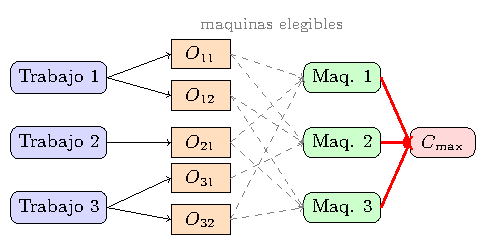
\includegraphics[width=\columnwidth]{fig_fjsp_diagram.pdf}
\caption{Esquema del FJSP: trabajos con operaciones asignables a
m\'aquinas elegibles (l\'ineas punteadas). Objetivo: minimizar
$C_{\max}$.}
\label{fig:fjsp_diagram}
\end{figure}

Formalmente, sea $J = \{J_1, \dots, J_n\}$ un conjunto de $n$
trabajos que deben procesarse sobre
$\mathcal{M} = \{1, \dots, m\}$ m\'aquinas.
Cada trabajo $J_j$ consta de $n_j$ operaciones
$O_{1j}, O_{2j}, \dots, O_{n_j j}$ que deben ejecutarse en orden
estricto.
Cada operaci\'on $O_{ij}$ puede asignarse a cualquier m\'aquina $k$
del subconjunto $M_{ij} \subseteq \mathcal{M}$, con tiempo de
procesamiento $p_{ijk} > 0$ que puede variar seg\'un la m\'aquina.
El objetivo es minimizar el makespan $C_{\max}$, respetando que cada
m\'aquina procesa a lo sumo una operaci\'on a la vez y que las
operaciones de cada trabajo respetan su orden de precedencia.

\section{Modelo matem\'atico}
\label{sec:modelo}

El FJSP puede formularse como un programa lineal entero mixto (MILP)
siguiendo la propuesta de Brandimarte~\cite{brandimarte1993},
implementada en AMPL.

\subsection{Variables de decisi\'on}

Las variables del modelo son: $x_{ijk} \in \{0,1\}$, que vale~1 si
la operaci\'on $j$ del trabajo $i$ se asigna a la m\'aquina $k$;
$s_{ij} \geq 0$, el tiempo de inicio de dicha operaci\'on;
$y_{ijkab} \in \{0,1\}$, que ordena dos operaciones en competencia
por una misma m\'aquina; y $C_{\max} \geq 0$, el makespan a
minimizar.

\subsection{Formulaci\'on}

\begin{align}
\min \quad & C_{\max} \label{eq:obj}\\
\text{s.a.}\quad
& \sum_{k \in M_{ij}} x_{ijk} = 1
  \quad \forall\, i \in I,\; j \in J_i \label{eq:asig}\\
& s_{ij} \geq s_{i,j-1}
  + \sum_{k} p_{i,j-1,k}\,x_{i,j-1,k}
  \label{eq:prec}\\
& s_{ij} + \sum_{k} p_{ijk}\,x_{ijk} \leq C_{\max}
  \label{eq:cmax}\\
& s_{ij} \geq s_{ab} + p_{abk}
  - B(1-y_{ijkab}) - B(2 - x_{ijk} - x_{abk})
  \label{eq:disj1}\\
& s_{ab} \geq s_{ij} + p_{ijk}
  - B\,y_{ijkab} - B(2 - x_{ijk} - x_{abk})
  \label{eq:disj2}
\end{align}

\noindent donde $B = \sum_{i,j,k} p_{ijk}$ es la constante
disyuntiva.
La restricci\'on~\eqref{eq:asig} garantiza la asignaci\'on \'unica
de cada operaci\'on; \eqref{eq:prec} impone la precedencia
intratrabajo; \eqref{eq:cmax} define el makespan; y
\eqref{eq:disj1}--\eqref{eq:disj2} evitan la solapaci\'on en cada
m\'aquina, activ\'andose solo cuando ambas operaciones se asignan a
la misma m\'aquina $k$ (t\'erminos $x_{ijk}$, $x_{abk}$).
La implementaci\'on en AMPL sigue la estructura de
Brandimarte~\cite{brandimarte1993} con conjuntos \texttt{I},
\texttt{K}, \texttt{J\{i in I\}} y \texttt{M\{i in I, j in J[i]\}}.

Dado que el modelo exacto solo es tratable para instancias
peque\~nas, el resto del trabajo se concentra en enfoques
metaheur\'isticos.

\section{Experimento Computacional}
\label{sec:metaheuristicas}

Cada integrante del grupo implement\'o una metaheur\'istica
distinta, todas aplicadas sobre el mismo problema e instancias.
A continuaci\'on se describen brevemente.
La Fig.~\ref{fig:metodologia} resume la metodolog\'ia de trabajo.

\begin{figure}[!t]
\centering
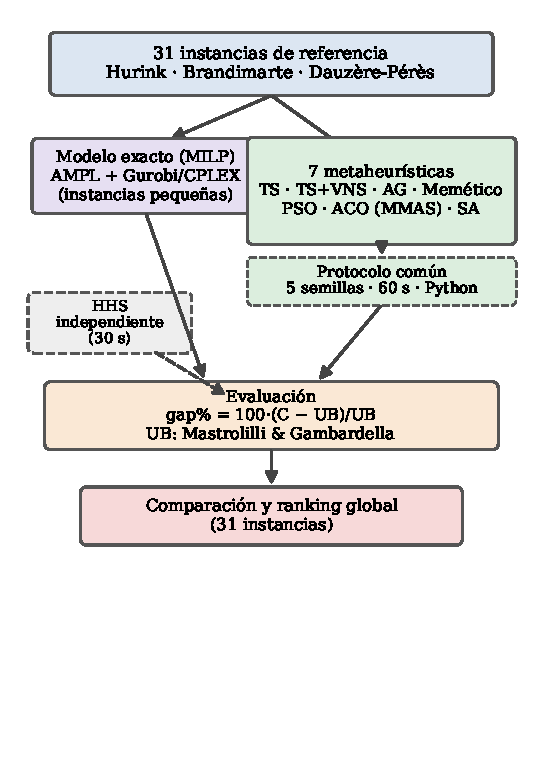
\includegraphics[width=0.92\columnwidth]{fig_metodologia.pdf}
\caption{Metodolog\'ia de trabajo: sobre un conjunto com\'un de 31
instancias se aplican dos enfoques ---un modelo exacto (MILP) y siete
metaheur\'isticas bajo un protocolo uniforme---, evaluados mediante el
gap\% respecto a la cota $UB$. La HHS se eval\'ua de forma
independiente.}
\label{fig:metodologia}
\end{figure}

\textbf{B\'usqueda Tab\'u (TS)~\cite{glover1986}.}
M\'etodo de trayectoria que explora el espacio de soluciones
movi\'endose de vecino en vecino manteniendo una lista tab\'u para
prohibir revisitar soluciones recientes, lo que permite escapar de
\'optimos locales. Se complementa con un criterio de aspiraci\'on.

\textbf{TS+VNS (h\'ibrida)~\cite{mladenovic1997}.}
Combina B\'usqueda Tab\'u con B\'usqueda de Vecindad Variable (VNS).
El VNS agita la soluci\'on incumbente cuando la TS se estanca; la
TS realiza la intensificaci\'on local. Emplea tres vecindarios con
agitaci\'on adaptativa.

\textbf{Algoritmo Gen\'etico (AG)~\cite{holland1975}.}
M\'etodo poblacional que evoluciona soluciones mediante operadores
de selecci\'on, cruzamiento y mutaci\'on, favoreciendo a los
individuos con menor makespan en cada generaci\'on.

\textbf{Algoritmo Mem\'etico~\cite{moscato1989}.}
H\'ibrido que combina un AG con b\'usqueda local basada en
elementos de TS. El refinamiento local de cada individuo acelera
la convergencia respecto a un AG puro.

\textbf{Optimizaci\'on por Enjambre de Part\'iculas
(PSO)~\cite{kennedy1995}.}
M\'etodo poblacional donde un conjunto de part\'iculas se desplaza
por el espacio de soluciones, guiadas por su mejor posici\'on
individual hist\'orica y la mejor posici\'on global del enjambre.

\textbf{Optimizaci\'on por Colonia de Hormigas (ACO,
MMAS)~\cite{dorigo1996,stutzle2000}.}
M\'etodo poblacional que construye soluciones probabil\'isticamente
guiado por rastros de feromona. La variante MMAS~\cite{stutzle2000}
acota los valores de feromona entre un l\'imite m\'inimo y m\'aximo
para evitar convergencia prematura.
Se utiliz\'o una tasa de evaporaci\'on de feromona del 10\% por
iteraci\'on ($\rho = 0.1$), conservando el 90\% del rastro
acumulado entre iteraciones, siguiendo las reglas del MAX-MIN Ant
System~\cite{stutzle2000}.

\textbf{Simulated Annealing (SA)~\cite{kirkpatrick1983}.}
M\'etodo de trayectoria inspirado en el recocido metal\'urgico.
Un vecino aleatorio se acepta si mejora la soluci\'on actual; si la
empeora, se acepta con probabilidad $e^{-\Delta/T}$, donde $\Delta$
es el deterioro y $T$ la temperatura, que decrece seg\'un un esquema
predefinido.

\textbf{B\'usqueda Arm\'onica H\'ibrida (HHS)~\cite{mahdavi2007}.}
Variante h\'ibrida de la B\'usqueda Arm\'onica, inspirada en la
improvisaci\'on musical. Una memoria arm\'onica almacena las mejores
soluciones y las nuevas se construyen combinando componentes de
dicha memoria con perturbaciones aleatorias. Esta metaheur\'istica
fue incorporada con posterioridad al protocolo experimental, por lo
que sus resultados se presentan de forma independiente
(Secci\'on~\ref{sec:hhs}).

En cuanto a la representaci\'on del problema, la mayor\'ia de los
m\'etodos poblacionales (AG, Mem\'etico, PSO) emplea una codificaci\'on
de dos vectores ---secuencia de operaciones y asignaci\'on de
m\'aquinas---, mientras que los m\'etodos de trayectoria (TS, TS+VNS,
SA) operan directamente sobre la soluci\'on mediante vecindarios.
La Tabla~\ref{tab:parametros} resume los par\'ametros principales y el
criterio de parada de cada metaheur\'istica.

\begin{table}[!t]
\caption{Par\'ametros principales y criterio de parada por
metaheur\'istica. Todas comparten el l\'imite de 60\,s por ejecuci\'on.}
\label{tab:parametros}
\centering
\footnotesize
\setlength{\tabcolsep}{3pt}
\renewcommand{\arraystretch}{1.2}
\begin{tabular}{@{}p{1.3cm}p{4.0cm}p{1.7cm}@{}}
\toprule
\textbf{Metaheur.} & \textbf{Par\'ametros principales}
  & \textbf{Criterio de parada} \\
\midrule
Tab\'u & Tenencia din\'amica $\sim\!\sqrt{n_{op}}$; 3 vecindarios;
  $\leq$300 vecinos/iter & 60\,s o 40 iter.\ sin mejora \\
TS+VNS & Tenencia 10; $k_{\max}=4$; 40 iteraciones
  & 60\,s \\
AG & Poblaci\'on 100; $p_c=0{,}9$; $p_m=0{,}2$; torneo $k=3$;
  elitismo 2 & 60\,s o 120 gen.\ sin mejora \\
Mem\'etico & Poblaci\'on 40; $p_c=0{,}9$; $p_m=0{,}2$; elitismo 2;
  b\'usqueda local (30 pruebas, $p_{ls}=0{,}5$) & 60\,s \\
PSO & Enjambre 40; $w: 0{,}9\!\to\!0{,}4$; $c_1=c_2=1{,}6$;
  $v_{\max}=0{,}3$ & 60\,s o 60 iter.\ sin mejora \\
ACO (MMAS) & 30 hormigas; $\alpha=1{,}0$; $\beta=2{,}0$;
  $\rho=0{,}1$; b\'usqueda local & 60\,s \\
SA & \emph{(por completar)} & 60\,s \\
\bottomrule
\end{tabular}
\end{table}

\section{Configuraci\'on computacional}
\label{sec:experimento}

\subsection{Protocolo com\'un}

Para garantizar la comparabilidad, todos los integrantes adoptaron
el mismo protocolo:

\begin{itemize}
  \item \textbf{Repeticiones:} 5 ejecuciones independientes por
        instancia.
  \item \textbf{Semillas:} 100, 101, 102, 103, 104 (fijas).
  \item \textbf{Tiempo l\'imite:} 60\,s por ejecuci\'on.
  \item \textbf{M\'etrica:}
        $\text{gap\%} = 100 \cdot (C_{\text{mejor}} - UB)/UB$,
        con $UB$ de Mastrolilli \&
        Gambardella~\cite{mastrolilli2000}.
  \item \textbf{Lenguaje:} Python.
\end{itemize}

\subsection{Instancias de prueba}

Las 31 instancias provienen de tres benchmarks cl\'asicos del FJSP,
resumidos en la Tabla~\ref{tab:instancias}.
Las cotas superiores de referencia fueron tomadas de Mastrolilli \&
Gambardella~\cite{mastrolilli2000}.
El benchmark de Barnes \& Chambers~\cite{barnes1996} se excluy\'o
por ser el menos referenciado en la literatura reciente de FJSP.

\begin{table}[!t]
\caption{Instancias seleccionadas por benchmark.}
\label{tab:instancias}
\centering
\small
\begin{tabular}{llccp{2.0cm}}
\toprule
\textbf{Benchmark} & \textbf{Inst.} & \textbf{T} & \textbf{M}
  & \textbf{Criterio} \\
\midrule
\multirow{5}{*}{\parbox{1.3cm}{Hurink\\(e/r/vdata)}}
  & la01 & 10 & 5  &
  \multirow{5}{2.0cm}{3 niveles de flexibilidad; $10{\times}5$
  a $15{\times}10$.} \\
  & la06 & 15 & 5  & \\
  & la11 & 20 & 5  & \\
  & la16 & 10 & 10 & \\
  & la21 & 15 & 10 & \\
\midrule
Brandimarte
  & Mk01--10 & 10--20 & 4--15
  & Las 10 instancias completas. \\
\midrule
\multirow{6}{*}{\parbox{1.3cm}{Dauz\`ere-\\P\'er\`es}}
  & 01a & 10 & 5  &
  \multirow{6}{2.0cm}{2 inst.\ por grupo ($10{\times}5$,
  $15{\times}8$, $20{\times}10$).} \\
  & 04a & 10 & 5  & \\
  & 07a & 15 & 8  & \\
  & 10a & 15 & 8  & \\
  & 13a & 20 & 10 & \\
  & 16a & 20 & 10 & \\
\bottomrule
\end{tabular}
\end{table}

\subsection{Justificaci\'on de la selecci\'on de instancias}

Los tres benchmarks seleccionados son los m\'as utilizados en la
literatura de FJSP y fueron adoptados por Mastrolilli \&
Gambardella~\cite{mastrolilli2000}, garantizando comparabilidad
directa con trabajos previos.
De Hurink se incluyeron las tres variantes de flexibilidad para
estudiar su efecto, seleccionando cinco instancias de $10{\times}5$
a $15{\times}10$.
Brandimarte se incluy\'o \'integro (Mk01--Mk10) por ser el benchmark
m\'as citado en comparaciones de FJSP.
La Fig.~\ref{fig:salida_mk} ilustra, de forma esquem\'atica, la
estructura de salida de una soluci\'on para estas instancias: cada
metaheur\'istica entrega una asignaci\'on de operaciones a m\'aquinas
representable como un diagrama de Gantt.

\begin{figure}[!t]
\centering
\begin{tikzpicture}[x=0.48cm, y=0.9cm, >=latex, font=\small]
  \node[anchor=east] at (-0.1, 1)   {MH1};
  \node[anchor=east] at (-0.1, 0)   {MH2};
  \draw[fill=gray!20] (-0.75, 0.55) rectangle (0, 1.45);
  \node at (-0.375, 1)  {\tiny\textbf{D}};
  \draw[fill=gray!20] (-0.75,-0.45) rectangle (0, 0.45);
  \node at (-0.375, 0)  {\tiny\textbf{D}};
  \filldraw[fill=blue!35,  draw=black, thick] (0.0, 0.55) rectangle (2.2, 1.45);
  \node at (1.1,  1) {\tiny $J_2 O_1$};
  \filldraw[fill=green!40, draw=black, thick] (2.2, 0.55) rectangle (4.1, 1.45);
  \node at (3.15, 1) {\tiny $J_1 O_2$};
  \filldraw[fill=orange!55,draw=black, thick] (4.1, 0.55) rectangle (5.8, 1.45);
  \node at (4.95, 1) {\tiny $J_3 O_1$};
  \filldraw[fill=red!35,   draw=black, thick] (0.0,-0.45) rectangle (2.5, 0.45);
  \node at (1.25, 0) {\tiny $J_1 O_1$};
  \filldraw[fill=violet!30,draw=black, thick] (2.5,-0.45) rectangle (3.9, 0.45);
  \node at (3.2,  0) {\tiny $J_3 O_2$};
  \filldraw[fill=yellow!60,draw=black, thick] (3.9,-0.45) rectangle (5.8, 0.45);
  \node at (4.85, 0) {\tiny $J_2 O_2$};
  \draw[->, thick] (-0.75,-0.75) -- (6.3,-0.75) node[right] {$t$};
  \draw (0,   -0.68) -- (0,   -0.82)  node[below] {\tiny $0$};
  \draw (5.8, -0.68) -- (5.8, -0.82)  node[below] {\tiny $C_{\max}$};
  \draw[dashed, gray] (-0.9, 0.5) -- (6.1, 0.5);
\end{tikzpicture}
\caption{Esquema de salida para las instancias Mk01--Mk10 del benchmark
Brandimarte. Cada fila representa una m\'aquina; los bloques coloreados
corresponden a operaciones asignadas por dos metaheur\'isticas distintas
(MH1, MH2). El makespan $C_{\max}$ es el criterio a minimizar.}
\label{fig:salida_mk}
\end{figure}

De Dauz\`ere-P\'er\`es se seleccionaron dos instancias por grupo
de tama\~no para representar la variabilidad sin incurrir en tiempo
de c\'omputo excesivo.
Barnes \& Chambers~\cite{barnes1996} se excluy\'o por ser el menos
referenciado en la literatura reciente.

\section{Resultados}
\label{sec:resultados}

\begin{figure*}[!t]
\centering
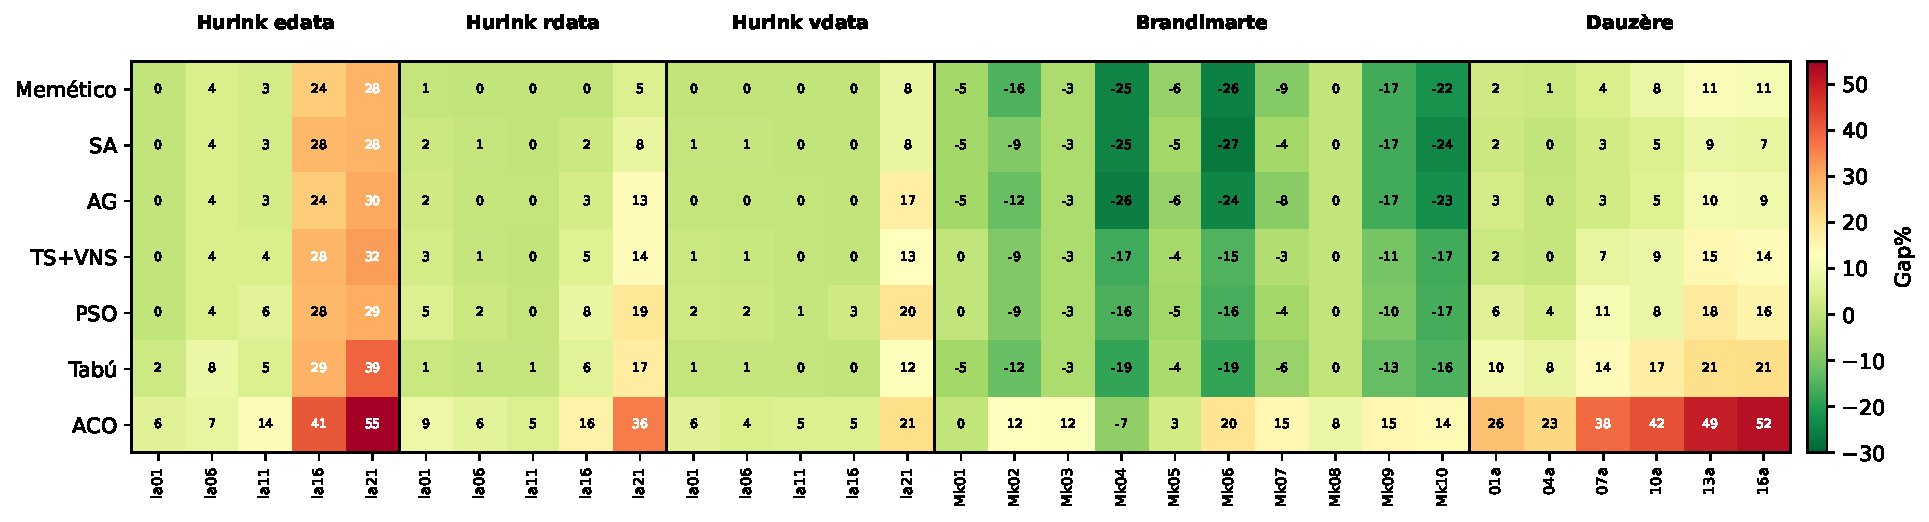
\includegraphics[width=\textwidth]{fig_heatmap_gap.pdf}
\caption{Mapa de calor del gap\% por instancia y metaheur\'istica.
Verde = buen desempe\~no; rojo = gap elevado.}
\label{fig:heatmap}
\end{figure*}

\begin{table*}[tp]
\caption{Mejor makespan (m\'in.\ sobre 5 repeticiones) por
instancia, para las ocho metaheur\'isticas evaluadas.
\textsuperscript{*}HHS usa un protocolo independiente
(30\,s/ejec.) y no es directamente comparable.}
\label{tab:hhs}
\centering
\scriptsize
\setlength{\tabcolsep}{4.5pt}
\begin{tabular}{llrrrrrrrrr}
\toprule
\textbf{Bench.} & \textbf{Inst.} & \textbf{UB} & \textbf{Mem\'et.}
  & \textbf{SA} & \textbf{AG} & \textbf{TS+VNS} & \textbf{PSO}
  & \textbf{Tab\'u} & \textbf{ACO} & \textbf{HHS\textsuperscript{*}} \\
\midrule
\multirow{5}{*}{\parbox{1.1cm}{Hurink\\edata}}
  & la01 & 609  & 609 & 609 & 609 & 609 & 609 & 621 & 644 & 612 \\
  & la06 & 800  & 833 & 833 & 833 & 833 & 833 & 866 & 859 & 836 \\
  & la11 & 1071 & 1104 & 1104 & 1106 & 1115 & 1134 & 1122 & 1218 & 1114 \\
  & la16 & 717  & 892 & 915 & 892 & 918 & 915 & 923 & 1010 & 921 \\
  & la21 & 835  & 1070 & 1071 & 1086 & 1100 & 1078 & 1162 & 1292 & 1120 \\
\midrule
\multirow{5}{*}{\parbox{1.1cm}{Hurink\\rdata}}
  & la01 & 570  & 573 & 580 & 584 & 587 & 598 & 577 & 620 & 578 \\
  & la06 & 799  & 799 & 804 & 801 & 805 & 812 & 804 & 850 & 803 \\
  & la11 & 1071 & 1071 & 1072 & 1076 & 1073 & 1076 & 1079 & 1126 & 1079 \\
  & la16 & 717  & 717 & 730 & 741 & 755 & 773 & 761 & 832 & 734 \\
  & la21 & 833  & 872 & 897 & 945 & 948 & 992 & 976 & 1132 & 966 \\
\midrule
\multirow{5}{*}{\parbox{1.1cm}{Hurink\\vdata}}
  & la01 & 570  & 571 & 574 & 572 & 578 & 581 & 573 & 602 & 575 \\
  & la06 & 799  & 800 & 806 & 802 & 807 & 812 & 804 & 832 & 806 \\
  & la11 & 1071 & 1071 & 1073 & 1076 & 1076 & 1079 & 1076 & 1125 & 1080 \\
  & la16 & 717  & 717 & 717 & 717 & 717 & 735 & 717 & 754 & 717 \\
  & la21 & 800  & 861 & 861 & 934 & 902 & 956 & 895 & 968 & 959 \\
\midrule
\multirow{10}{*}{Brand.}
  & Mk01 & 42  & 40 & 40 & 40 & 42 & 42 & 40 & 42 & 41 \\
  & Mk02 & 32  & 27 & 29 & 28 & 29 & 29 & 28 & 36 & 29 \\
  & Mk03 & 211 & 204 & 204 & 204 & 204 & 204 & 204 & 236 & 204 \\
  & Mk04 & 81  & 61 & 61 & 60 & 67 & 68 & 66 & 75 & 65 \\
  & Mk05 & 186 & 174 & 177 & 174 & 178 & 177 & 179 & 191 & 176 \\
  & Mk06 & 86  & 64 & 63 & 65 & 73 & 72 & 70 & 103 & 73 \\
  & Mk07 & 157 & 143 & 150 & 144 & 153 & 150 & 147 & 180 & 146 \\
  & Mk08 & 523 & 523 & 523 & 523 & 523 & 523 & 523 & 566 & 523 \\
  & Mk09 & 369 & 307 & 307 & 307 & 330 & 333 & 322 & 423 & 325 \\
  & Mk10 & 296 & 230 & 224 & 228 & 246 & 247 & 250 & 337 & 273 \\
\midrule
\multirow{6}{*}{Dauz\`ere}
  & 01a & 2530 & 2593 & 2574 & 2610 & 2568 & 2675 & 2778 & 3192 & 2750 \\
  & 04a & 2565 & 2602 & 2565 & 2576 & 2575 & 2655 & 2762 & 3147 & 2714 \\
  & 07a & 2408 & 2506 & 2474 & 2470 & 2582 & 2665 & 2739 & 3329 & 2711 \\
  & 10a & 2362 & 2549 & 2475 & 2488 & 2563 & 2554 & 2760 & 3349 & 2789 \\
  & 13a & 2302 & 2560 & 2498 & 2533 & 2638 & 2714 & 2782 & 3439 & 2719 \\
  & 16a & 2301 & 2550 & 2470 & 2517 & 2618 & 2665 & 2794 & 3491 & 2698 \\
\bottomrule
\end{tabular}
\end{table*}

\begin{figure*}[!t]
\centering
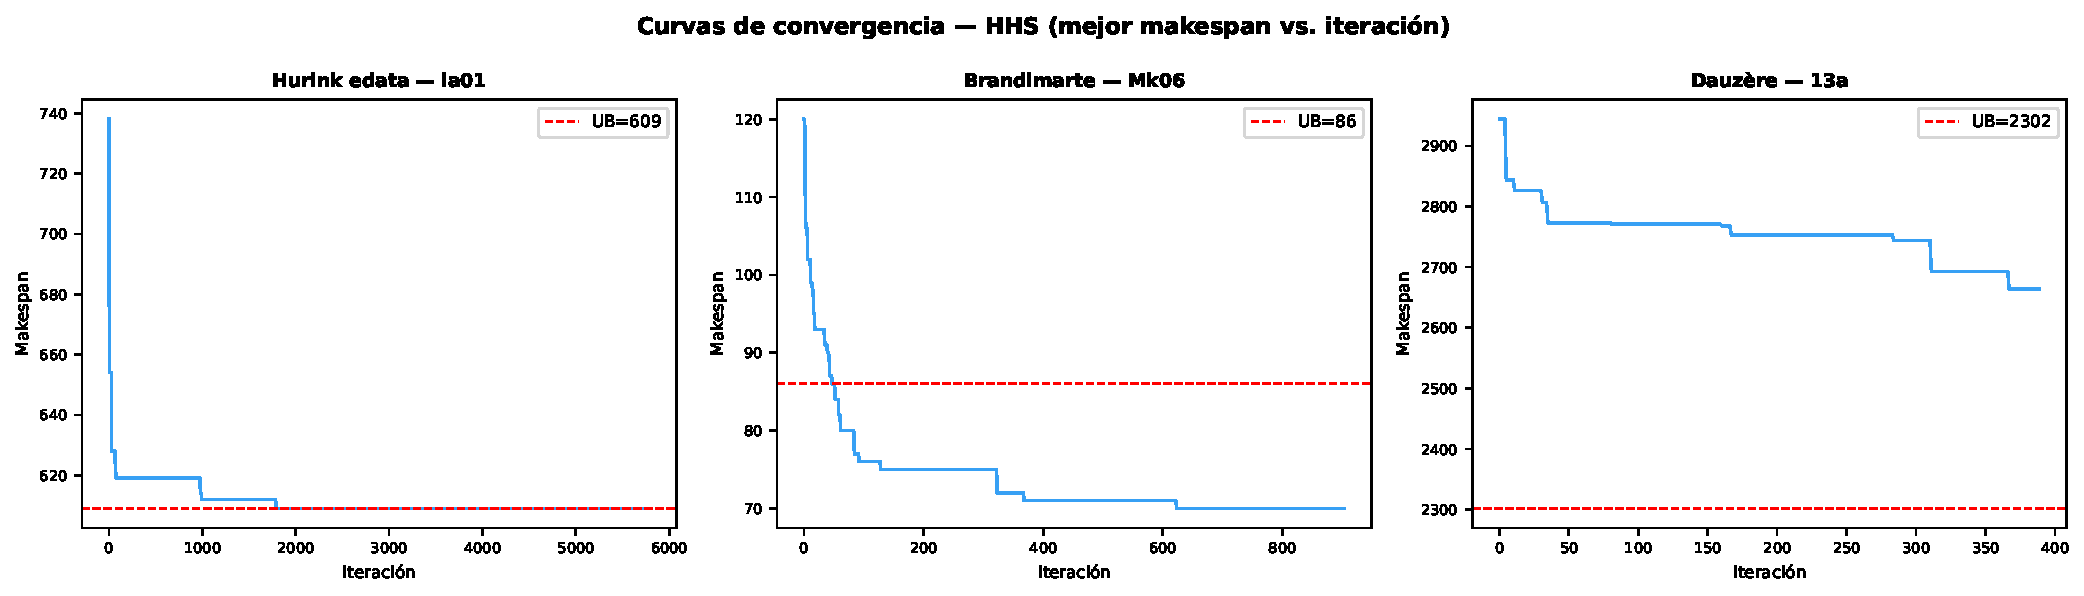
\includegraphics[width=\textwidth]{fig_conv_hhs.pdf}
\caption{Curvas de convergencia del HHS en tres instancias
representativas. La l\'inea roja punteada indica la cota $UB$
propia del HHS.}
\label{fig:conv_hhs}
\end{figure*}

La Tabla~\ref{tab:resultados} presenta el gap\% del mejor makespan
(BKS sobre 5 repeticiones) respecto a la cota $UB$ para cada
benchmark.
Valores negativos indican que la metaheur\'istica super\'o la cota
reportada en la literatura, lo que ocurre especialmente en
Brandimarte debido al avance del hardware en 25~a\~nos.
La Fig.~\ref{fig:ranking} resume el ranking global y la
Fig.~\ref{fig:heatmap} muestra el detalle completo por instancia.

\begin{table}[!t]
\caption{Gap\% del BKS por benchmark. Valores negativos indican
superaci\'on de la cota de Mastrolilli \&
Gambardella~\cite{mastrolilli2000}. En negrita: mejor valor de
cada columna.}
\label{tab:resultados}
\centering
\scriptsize
\setlength{\tabcolsep}{2.3pt}
\begin{tabular}{lcccccc}
\toprule
\textbf{Metaheur\'istica}
  & \textbf{edata} & \textbf{rdata} & \textbf{vdata}
  & \textbf{Brand.} & \textbf{Dauz.}
  & \textbf{Global} \\
\midrule
Mem\'etico  & \textbf{11.95} & \textbf{1.04} & \textbf{1.59}
  & $\mathbf{-12.84}$ & 6.32 & $\mathbf{-0.57}$ \\
SA          & 12.62 & 2.39 & 1.88
  & $-11.93$ & \textbf{4.19} & $-0.31$ \\
AG          & 12.37 & 3.99 & 3.59
  & $-12.54$ & 5.15 & $0.17$ \\
TS+VNS      & 13.57 & 4.61 & 3.12
  & $-7.94$  & 7.67 & $2.36$ \\
PSO         & 13.34 & 6.78 & 5.26
  & $-8.06$  & 10.29 & $3.49$ \\
Tab\'u      & 16.57 & 5.18 & 2.70
  & $-9.61$  & 15.06 & $3.76$ \\
ACO         & 24.49 & 14.44 & 8.19
  & $9.09$   & 38.30 & $17.95$ \\
\bottomrule
\end{tabular}
\end{table}

\begin{figure}[!t]
\centering
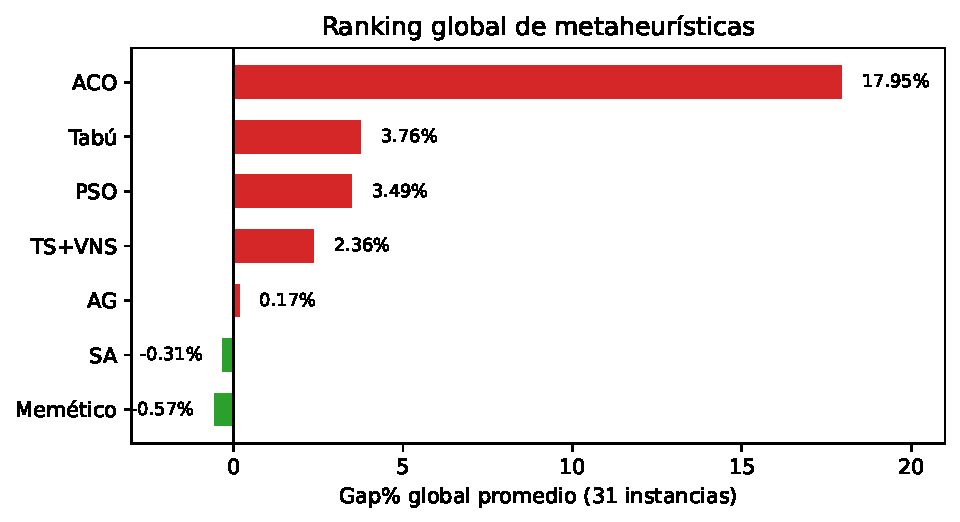
\includegraphics[width=\columnwidth]{fig_ranking_global.pdf}
\caption{Ranking global por gap\% promedio sobre las 31 instancias.
Valores negativos indican superaci\'on de la cota de referencia.}
\label{fig:ranking}
\end{figure}

\subsection{Resultados adicionales: HHS}
\label{sec:hhs}

La metaheur\'istica HHS fue incorporada con posterioridad al
dise\~no del protocolo experimental com\'un.
Sus experimentos se realizaron con un tiempo l\'imite de 30\,s por
ejecuci\'on y cotas de referencia provenientes de una fuente
distinta a Mastrolilli \& Gambardella~\cite{mastrolilli2000}
---por ejemplo, $UB(\text{Mk01})=40$ y $UB(\text{Mk10})=193$
frente a los valores 42 y 296 del resto del grupo---, por lo que
sus resultados no son directamente comparables.
La Tabla~\ref{tab:hhs} presenta el mejor makespan obtenido por cada
metaheur\'istica en cada instancia, y la Fig.~\ref{fig:conv_hhs}
muestra las curvas de convergencia en tres instancias
representativas.

\section{Discusi\'on}
\label{sec:discusion}

Los resultados de la Tabla~\ref{tab:resultados} y la
Fig.~\ref{fig:ranking} permiten ordenar las siete metaheur\'isticas
de mejor a peor desempe\~no global.
El Algoritmo Mem\'etico lidera con un gap global de $-0.57\%$,
superando en promedio las cotas de referencia de
Mastrolilli \& Gambardella~\cite{mastrolilli2000}.
El SA ocupa el segundo lugar ($-0.31\%$), seguido por el AG
($+0.17\%$).
El ACO queda claramente por debajo ($+17.95\%$), con dificultades
especialmente marcadas en Dauz\`ere ($+38.30\%$).

El mapa de calor de la Fig.~\ref{fig:heatmap} revela tres patrones
consistentes:

\begin{enumerate}
  \item \textbf{La flexibilidad facilita el problema.}
        En todas las metaheur\'isticas el gap disminuye al pasar de
        edata (baja flexibilidad) a vdata (alta flexibilidad).

  \item \textbf{Los h\'ibridos dominan.}
        El Mem\'etico y el TS+VNS figuran sistem\'aticamente entre
        los mejores. El SA tambi\'en destaca gracias a su mecanismo
        de aceptaci\'on probabil\'istica.

  \item \textbf{Superaci\'on de cotas en Brandimarte.}
        Seis de las siete metaheur\'isticas obtienen gaps negativos,
        reflejo del avance del hardware en 25~a\~nos y la naturaleza
        de cota superior (no \'optimo) de esos valores.
\end{enumerate}

El caso del ACO (MMAS) sugiere que la calidad de la implementaci\'on
y el ajuste de par\'ametros son tan determinantes como la elecci\'on
del algoritmo.

Respecto al HHS, sus curvas de convergencia (Fig.~\ref{fig:conv_hhs})
muestran convergencia r\'apida en instancias peque\~nas, con
dificultades en la21 y en las instancias m\'as grandes de Dauz\`ere.

\section{Conclusiones}
\label{sec:conclusiones}

Se implementaron y compararon siete metaheur\'isticas para el FJSP
sobre 31 instancias de tres benchmarks cl\'asicos, bajo un protocolo
experimental uniforme.
El Algoritmo Mem\'etico obtuvo el mejor desempe\~no global
($\text{gap\%} = -0.57$), seguido por el SA~($-0.31$) y el
AG~($+0.17$).
Los dos primeros superaron en promedio las cotas de
Mastrolilli \& Gambardella~\cite{mastrolilli2000}; el AG obtuvo
un gap pr\'acticamente nulo.
El ACO present\'o los resultados menos competitivos, en particular
en Dauz\`ere.
Seis de los siete m\'etodos superaron las cotas en Brandimarte,
reflejo del avance del hardware desde el a\~no~2000.
La HHS, evaluada de forma independiente (30\,s), mostr\'o resultados
prometedores en instancias peque\~nas de Hurink y mayores
dificultades a medida que crece el tama\~no del problema.

Como trabajo futuro se plantea la comparaci\'on con un solver exacto
(Gurobi o CPLEX) en instancias de menor tama\~no, lo que permitir\'ia
medir la distancia al \'optimo real.

\section*{Declaraci\'on de uso de IA}

En la elaboraci\'on de este trabajo se utilizaron herramientas de
inteligencia artificial generativa (Claude, Anthropic) como apoyo
en las siguientes tareas: generaci\'on y depuraci\'on de c\'odigo
Python para la implementaci\'on de las metaheur\'isticas,
procesamiento y visualizaci\'on de resultados experimentales,
formateo del documento en \LaTeX{} bajo la plantilla IEEE, y
revisi\'on ortogr\'afica y gramatical del texto.
El dise\~no algor\'itmico, la configuraci\'on de par\'ametros, la
ejecuci\'on de experimentos y el an\'alisis e interpretaci\'on de
los resultados fueron realizados \'integramente por los autores.


\balance
\begin{thebibliography}{25}

\bibitem{hurink1994}
E.~Hurink, B.~Jurisch, and M.~Thole,
``Tabu search for the job-shop scheduling problem with multi-purpose
machines,''
\textit{OR Spektrum}, vol.~15, pp.~205--215, 1994.

\bibitem{mastrolilli2000}
M.~Mastrolilli and L.\,M.~Gambardella,
``Effective neighborhood functions for the flexible job shop problem,''
\textit{Journal of Scheduling}, vol.~3, no.~1, pp.~3--20, 2000.

\bibitem{brandimarte1993}
P.~Brandimarte,
``Routing and scheduling in a flexible job shop by tabu search,''
\textit{Annals of Operations Research}, vol.~41, pp.~157--183, 1993.

\bibitem{dauzere1997}
S.~Dauz\`ere-P\'er\`es and J.~Paulli,
``An integrated approach for modeling and solving the general
multiprocessor job-shop scheduling problem using tabu search,''
\textit{Annals of Operations Research}, vol.~70, pp.~281--306, 1997.

\bibitem{glover1986}
F.~Glover,
``Future paths for integer programming and links to artificial
intelligence,''
\textit{Computers \& Operations Research}, vol.~13, no.~5,
pp.~533--549, 1986.

\bibitem{mladenovic1997}
N.~Mladenovi\'c and P.~Hansen,
``Variable neighborhood search,''
\textit{Computers \& Operations Research}, vol.~24, no.~11,
pp.~1097--1100, 1997.

\bibitem{barnes1996}
J.\,W.~Barnes and J.\,B.~Chambers,
``Flexible job shop scheduling by tabu search,''
Technical Report ORP96-09, Univ.\ of Texas at Austin, 1996.

\bibitem{garey1976}
M.\,R.~Garey, D.\,S.~Johnson, and R.~Sethi,
``The complexity of flowshop and jobshop scheduling,''
\textit{Mathematics of Operations Research}, vol.~1, no.~2,
pp.~117--129, 1976.

\bibitem{garey1979}
M.\,R.~Garey and D.\,S.~Johnson,
\textit{Computers and Intractability: A Guide to the Theory of
NP-Completeness}.
New York: W.\,H.~Freeman, 1979.

\bibitem{holland1975}
J.\,H.~Holland,
\textit{Adaptation in Natural and Artificial Systems}.
Ann Arbor: University of Michigan Press, 1975.

\bibitem{moscato1989}
P.~Moscato,
``On evolution, search, optimization, genetic algorithms and martial
arts: Towards memetic algorithms,''
Tech.\ Rep.\ 826, Caltech Concurrent Computation Program, 1989.

\bibitem{kennedy1995}
J.~Kennedy and R.~Eberhart,
``Particle swarm optimization,''
in \textit{Proc.\ ICNN'95}, Perth, 1995, pp.~1942--1948.

\bibitem{dorigo1996}
M.~Dorigo, V.~Maniezzo, and A.~Colorni,
``Ant system: Optimization by a colony of cooperating agents,''
\textit{IEEE Trans.\ Syst., Man, Cybern.\ B}, vol.~26, no.~1,
pp.~29--41, 1996.

\bibitem{stutzle2000}
T.~St\"utzle and H.\,H.~Hoos,
``MAX-MIN ant system,''
\textit{Future Generation Computer Systems}, vol.~16, no.~8,
pp.~889--914, 2000.

\bibitem{kirkpatrick1983}
S.~Kirkpatrick, C.\,D.~Gelatt, and M.\,P.~Vecchi,
``Optimization by simulated annealing,''
\textit{Science}, vol.~220, no.~4598, pp.~671--680, 1983.

\bibitem{mahdavi2007}
M.~Mahdavi, M.~Fesanghary, and E.~Damangir,
``An improved harmony search algorithm for solving optimization
problems,''
\textit{Applied Mathematics and Computation}, vol.~188, no.~2,
pp.~1567--1579, 2007.

\bibitem{pinedo2012}
M.\,L.~Pinedo,
\textit{Scheduling: Theory, Algorithms, and Systems}, 4th~ed.
New York: Springer, 2012.

\bibitem{brucker2007}
P.~Brucker,
\textit{Scheduling Algorithms}, 5th~ed.
Berlin: Springer, 2007.

\bibitem{pezzella2008}
F.~Pezzella, G.~Morganti, and G.~Ciaschetti,
``A genetic algorithm for the flexible job-shop scheduling problem,''
\textit{Computers \& Operations Research}, vol.~35, no.~10,
pp.~3202--3212, 2008.

\bibitem{xia2005}
W.~Xia and Z.~Wu,
``An effective hybrid optimization approach for multi-objective
flexible job-shop scheduling problems,''
\textit{Computers \& Industrial Engineering}, vol.~48, no.~2,
pp.~409--425, 2005.

\bibitem{zhang2009}
G.~Zhang, X.~Shao, P.~Li, and L.~Gao,
``An effective hybrid particle swarm optimization algorithm for
multi-objective flexible job-shop scheduling problem,''
\textit{Computers \& Industrial Engineering}, vol.~56, no.~4,
pp.~1309--1318, 2009.

\bibitem{li2016}
X.~Li and L.~Gao,
``An effective hybrid genetic algorithm and tabu search for flexible
job shop scheduling problem,''
\textit{Int.\ J.\ Production Economics}, vol.~174,
pp.~93--110, 2016.

\bibitem{dreo2006}
J.~Dr\'eo, A.~P\'etrowski, P.~Siarry, and E.~Taillard,
\textit{Metaheuristics for Hard Optimization}.
Berlin: Springer, 2006.

\bibitem{lawler1993}
E.\,L.~Lawler, J.\,K.~Lenstra, A.\,H.\,G.~Rinnooy~Kan, and
D.\,B.~Shmoys,
``Sequencing and scheduling: Algorithms and complexity,''
in \textit{Handbooks in Operations Research}, vol.~4.
Amsterdam: Elsevier, 1993, pp.~445--522.

\bibitem{gatica2011}
G.~Gatica and R.\,R.~Gonz\'alez,
``Metaheur\'isticas aplicadas a problemas de scheduling en sistemas
de manufactura flexible,''
\textit{Ingeniare. Revista chilena de ingenier\'ia}, vol.~19,
no.~1, pp.~74--85, 2011.

% Requiere en el preambulo: \usepackage{multirow}
\begin{table*}[tp]
\caption{Resultados por instancia: mejor makespan ($C_{\max}$) y tiempo de c\'omputo $T$(s) del modelo exacto (AMPL/Gurobi, l\'imite de 60\,s por instancia) y de las ocho metaheur\'isticas evaluadas. BKS: mejor soluci\'on conocida. En negrita: mejor valor entre las siete metaheur\'isticas del protocolo com\'un. ``---'' indica que no se encontr\'o soluci\'on factible dentro del l\'imite de tiempo. \textsuperscript{*}HHS usa un protocolo independiente y se reporta como referencia.}
\label{tab:resultados_completos}
\centering\scriptsize
\setlength{\tabcolsep}{2.6pt}
\begin{tabular}{lr rr rr rr rr rr rr rr rr rr}
\hline
\multirow{2}{*}{Instancia} & \multirow{2}{*}{BKS} & \multicolumn{2}{c}{AMPL} & \multicolumn{2}{c}{AG} & \multicolumn{2}{c}{ACO} & \multicolumn{2}{c}{MH-K} & \multicolumn{2}{c}{MEM} & \multicolumn{2}{c}{PSO} & \multicolumn{2}{c}{TS} & \multicolumn{2}{c}{TS+VNS} & \multicolumn{2}{c}{HHS\textsuperscript{*}} \\
 &  & $C_{\max}$ & $T$(s) & $C_{\max}$ & $T$(s) & $C_{\max}$ & $T$(s) & $C_{\max}$ & $T$(s) & $C_{\max}$ & $T$(s) & $C_{\max}$ & $T$(s) & $C_{\max}$ & $T$(s) & $C_{\max}$ & $T$(s) & $C_{\max}$ & $T$(s) \\
\hline
\multicolumn{20}{l}{\emph{Brandimarte}} \\
Mk01 & 40 & 40 & 60 & \textbf{40} & 60 & 42 & 60 & \textbf{40} & 6 & \textbf{40} & 60 & 42 & 60 & \textbf{40} & 60 & 42 & 6.6 & 40 & 7.6 \\
Mk02 & 26 & 27 & 60 & 28 & 60 & 36 & 60 & 29 & 6.3 & \textbf{27} & 60 & 29 & 60 & 28 & 60 & 29 & 7.2 & 28 & 23.9 \\
Mk03 & 204 & 242 & 60 & \textbf{204} & 60 & 236 & 60 & \textbf{204} & 56.5 & \textbf{204} & 60 & \textbf{204} & 60.1 & \textbf{204} & 60 & \textbf{204} & 16.9 & 204 & 30 \\
Mk04 & 60 & 63 & 60 & \textbf{60} & 60 & 75 & 60 & 61 & 18.5 & 61 & 60 & 68 & 60 & 66 & 60 & 67 & 11.1 & 62 & 23.8 \\
Mk05 & 172 & 189 & 60 & \textbf{174} & 60 & 191 & 60 & 177 & 32.9 & \textbf{174} & 60 & 177 & 60 & 179 & 60 & 178 & 13.6 & 175 & 30 \\
Mk06 & 57 & 100 & 60 & 65 & 60 & 103 & 60 & \textbf{63} & 51.5 & 64 & 60.1 & 72 & 60.1 & 70 & 60 & 73 & 17.9 & 70 & 30 \\
Mk07 & 139 & 165 & 60 & 144 & 60 & 180 & 60 & 150 & 30.2 & \textbf{143} & 60 & 150 & 60 & 147 & 60 & 153 & 12.4 & 144 & 30 \\
Mk08 & 523 & 549 & 60 & \textbf{523} & 60 & 566 & 60 & \textbf{523} & 174.3 & \textbf{523} & 60 & \textbf{523} & 60.1 & \textbf{523} & 60 & \textbf{523} & 26 & 523 & 30 \\
Mk09 & 307 & --- & 60 & \textbf{307} & 60 & 423 & 60 & \textbf{307} & 170.7 & \textbf{307} & 60 & 333 & 60.1 & 322 & 60 & 330 & 29.6 & 318 & 30 \\
Mk10 & 193 & --- & 60 & 228 & 60 & 337 & 60 & \textbf{224} & 158.9 & 230 & 60.1 & 247 & 60.2 & 250 & 60 & 246 & 29.6 & 266 & 30 \\
\hline
\multicolumn{20}{l}{\emph{Dauz\`ere-P\'er\`es y Paulli}} \\
01a & 2505 & 2942 & 60 & 2610 & 60 & 3192 & 60 & 2574 & 167.5 & 2593 & 60 & 2675 & 60.2 & 2778 & 60 & \textbf{2568} & 27.9 & 2686 & 30 \\
04a & 2503 & 2998 & 60 & 2576 & 60 & 3147 & 60 & \textbf{2565} & 159.1 & 2602 & 60 & 2655 & 60.1 & 2762 & 60 & 2575 & 25.6 & 2687 & 30 \\
07a & 2254 & 3058 & 60 & \textbf{2470} & 60 & 3329 & 60 & 2474 & 363 & 2506 & 60 & 2665 & 60.1 & 2739 & 60 & 2582 & 42.2 & 2679 & 30 \\
10a & 2241 & 3278 & 60 & 2488 & 60 & 3349 & 60 & \textbf{2475} & 348.9 & 2549 & 60 & 2554 & 60.1 & 2760 & 60.1 & 2563 & 44.8 & 2652 & 30 \\
13a & 2236 & 28735 & 60 & 2533 & 60 & 3439 & 60 & \textbf{2498} & 667.8 & 2560 & 60.1 & 2714 & 60.2 & 2782 & 60.1 & 2638 & 60.5 & 2664 & 30 \\
16a & 2231 & --- & 60 & 2517 & 60 & 3491 & 60 & \textbf{2470} & 666.2 & 2550 & 60.1 & 2665 & 60.4 & 2794 & 60.1 & 2618 & 60.8 & 2667 & 30 \\
\hline
\multicolumn{20}{l}{\emph{Hurink \emph{edata}}} \\
la01 & 609 & 609 & 60 & \textbf{609} & 60 & 644 & 60 & \textbf{609} & 6.9 & \textbf{609} & 60 & \textbf{609} & 60 & 621 & 60 & \textbf{609} & 6 & 609 & 5.8 \\
la06 & 833 & 833 & 60 & \textbf{833} & 60 & 859 & 60 & \textbf{833} & 17.8 & \textbf{833} & 60 & \textbf{833} & 60 & 866 & 60 & \textbf{833} & 8.5 & 833 & 15.2 \\
la11 & 1103 & 1106 & 60 & 1106 & 60 & 1218 & 60 & \textbf{1104} & 33.9 & \textbf{1104} & 60 & 1134 & 60 & 1122 & 60 & 1115 & 11.5 & 1106 & 29.6 \\
la16 & 892 & 892 & 60 & \textbf{892} & 60 & 1010 & 60 & 915 & 27.9 & \textbf{892} & 60 & 915 & 60 & 923 & 60 & 918 & 11.6 & 917 & 13.6 \\
la21 & 1009 & 1066 & 60 & 1086 & 60 & 1292 & 60 & 1071 & 66.5 & \textbf{1070} & 60 & 1078 & 60 & 1162 & 60 & 1100 & 18.4 & 1100 & 30 \\
\hline
\multicolumn{20}{l}{\emph{Hurink \emph{rdata}}} \\
la01 & 570 & 577 & 60 & 584 & 60 & 620 & 60 & 580 & 7.6 & \textbf{573} & 60 & 598 & 60 & 577 & 60 & 587 & 5.9 & 575 & 12.8 \\
la06 & 799 & 806 & 60 & 801 & 60 & 850 & 60 & 804 & 17.9 & \textbf{799} & 60 & 812 & 60 & 804 & 60 & 805 & 8.7 & 800 & 29.3 \\
la11 & 1071 & 1096 & 60 & 1076 & 60 & 1126 & 60 & 1072 & 37.6 & \textbf{1071} & 60 & 1076 & 60 & 1079 & 60 & 1073 & 11.7 & 1075 & 30 \\
la16 & 717 & 717 & 60 & 741 & 60 & 832 & 60 & 730 & 29.2 & \textbf{717} & 60 & 773 & 60 & 761 & 60 & 755 & 13.1 & 717 & 29.9 \\
la21 & 825 & 890 & 60 & 945 & 60 & 1132 & 60 & 897 & 73.6 & \textbf{872} & 60 & 992 & 60 & 976 & 60 & 948 & 20.3 & 932 & 30 \\
\hline
\multicolumn{20}{l}{\emph{Hurink \emph{vdata}}} \\
la01 & 570 & 573 & 60 & 572 & 60 & 602 & 60 & 574 & 6.6 & \textbf{571} & 60 & 581 & 60 & 573 & 60 & 578 & 6.5 & 572 & 20.5 \\
la06 & 799 & 803 & 60 & 802 & 60 & 832 & 60 & 806 & 17.7 & \textbf{800} & 60 & 812 & 60 & 804 & 60 & 807 & 9.4 & 802 & 30 \\
la11 & 1071 & 1098 & 60 & 1076 & 60 & 1125 & 60 & 1073 & 35.5 & \textbf{1071} & 60 & 1079 & 60 & 1076 & 60 & 1076 & 12.9 & 1076 & 30 \\
la16 & 717 & 717 & 60 & \textbf{717} & 60 & 754 & 60 & \textbf{717} & 28 & \textbf{717} & 60 & 735 & 60 & \textbf{717} & 60 & \textbf{717} & 13.3 & 717 & 30 \\
la21 & 800 & --- & 60 & 934 & 60 & 968 & 60 & \textbf{861} & 70.8 & \textbf{861} & 60 & 956 & 60.1 & 895 & 60 & 902 & 18.8 & 937 & 30 \\
\hline
\end{tabular}
\end{table*}
\end{thebibliography}

\end{document}